\documentclass[12pt]{article}
\usepackage[utf8]{inputenc}
\usepackage[english]{babel}
\usepackage{float}
\usepackage{pythonhighlight}
\usepackage{graphicx}

\renewcommand{\baselinestretch}{1.3}

\usepackage{biblatex}
\addbibresource{cw2.bib}


\newcommand{\numpy}{{\tt numpy}}    % tt font for numpy

\topmargin -.5in
\textheight 9in
\oddsidemargin -.25in
\evensidemargin -.25in
\textwidth 7in

\begin{document}

% ========== Edit your name here
\author{Baran Buluttekin\\13153116}
\title{Data Science Techniques and Applications\\Coursework II}
\date{March 23, 2019}
\maketitle

\medskip

\indent We can start of our analysis by getting the dataset. Corresponding Heart Diseases dataset\cite{kaggle}\cite{uci-source} can be downloaded from kaggle by clicking download link in the website. When the download finished we received compressed version of file named \textit{heart-disese-uci.zip}. Fallowing the un-compression of the file we will obtain csv file \textit{heart.csv} which is in final format for analysis. 

Next step is to loading python libraries to start the analysis. In this coursework fallowing open source libraries used:
\begin{enumerate}
    \item \textbf{Pandas: }Tabular data manipulation library that will be use to load the data and cleaning/reshaping.\cite{mckinney-proc-scipy-2010}
    \item \textbf{Matplotlib: }Will be used as main plotting library that has many pre build high level plotting tools.\cite{matplotlib}
    \item \textbf{Seaborn: }Python library for special plotting styles such as pairplots.\cite{seaborn}
    \item \textbf{Scikit-Learn: }Open source machine learning library that includes various machine learning algorithms.\cite{scikit-learn}
\end{enumerate}

As a first step libraries above loaded in python in the fallowing format.

\begin{python}
    import pandas as pd
    import matplotlib.pyplot as plt
    from mpl_toolkits.mplot3d import Axes3D
    from sklearn.decomposition import PCA
    import seaborn as sns
\end{python}

With the help of pandas library we can load the dataset and view first 5 rows to check if the data frame is in expected format.

\begin{python}
    df = pd.read_csv("heart.csv")
    df.head()
\end{python}

\begin{table}[h!]
    \centering
     \begin{tabular}{||c c c c c c c c c c c c c c||} 
     \hline
     age & sex & cp & trestbps & chol & fbs &restecg & thalach & exang & oldpeak & slope & ca & thal & target \\ [0.5ex] 
     \hline\hline
     63.0 & 1.0 & 3.0 & 145.0 & 233.0 & 1.0 & 0.0 & 150.0 & 0.0 & 2.3 & 0.0 & 0.0 & 1.0 & 1.0\\ 
     37.0 & 1.0 & 2.0 & 130.0 & 250.0 & 0.0 & 1.0 & 187.0 & 0.0 & 3.5 & 0.0 & 0.0 & 2.0 & 1.0\\
     41.0 & 0.0 & 1.0 & 130.0 & 204.0 & 0.0 & 0.0 & 172.0 & 0.0 & 1.4 & 2.0 & 0.0 & 2.0 & 1.0\\
     56.0 & 1.0 & 1.0 & 120.0 & 236.0 & 0.0 & 1.0 & 178.0 & 0.0 & 0.8 & 2.0 & 0.0 & 2.0 & 1.0\\
     57.0 & 0.0 & 0.0 & 120.0 & 354.0 & 0.0 & 1.0 & 163.0 & 1.0 & 0.6 & 2.0 & 0.0 & 2.0 & 1.0\\ [1ex] 
     \hline
     \end{tabular}
    \end{table}

Fallowing the guide of coursework, I choose "age", "chol" and "trestbps" as important dimensions. Description of the columns from the coursework I is given below as a reminder.

\begin{quote}
    \begin{enumerate}
        \item \textbf{age}: Age in years (max:77, min:29)
        \item \textbf{chol}: cholesterol level (mg/dl)
        \item \textbf{trestbps}: Blood pressure recording for resting
    \end{enumerate}
\end{quote}

In order to get a better grasp of the data distribution with these three variables, I will use pairplot. Pairplot will help us see different variation of these three variable with each other and with relation to the target outcome of the dataset.

\begin{python}
    selected_dims = ["age", "chol", "trestbps", "target"]
    sns.pairplot(df[selected_dims], hue="target")
\end{python}

\begin{figure}[H]
    \centering
    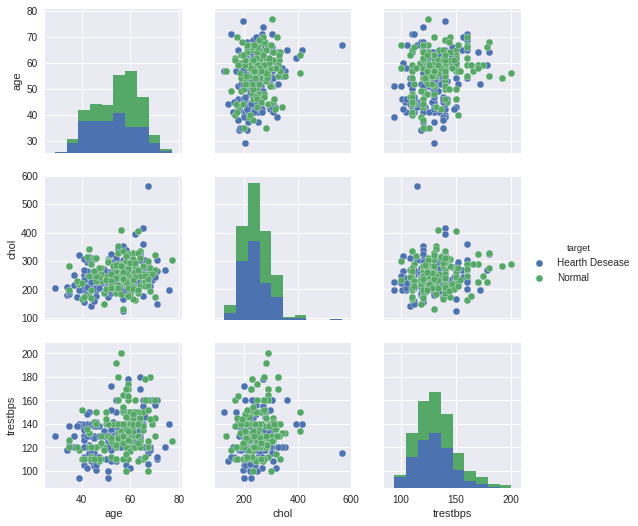
\includegraphics[width=\textwidth]{img/pairplot.png}
    \caption{Pairplot with chosen dimensions.}
\end{figure}
 
We can also plot these 3 dimensions in 3D plot to see their relation to target variable. I created helper function quickly plot 3D plots given dimensions in dataset. Code for the function follows.

\begin{python}
    def plot_3d(dataframe, x_label, y_label, z_label, target_label, title):
        labelTups = [("Normal", 0), ("Hearth Desease", 1)]
        fig = plt.figure(1, figsize=(8, 6))
        ax = Axes3D(fig, elev=-150, azim=110)
        ax.scatter(dataframe[x_label], dataframe[y_label], dataframe[z_label], c=dataframe[target_label],
                    cmap=plt.cm.Set1, edgecolor='k', s=40)
        ax.set_title(title)
        ax.set_xlabel(x_label)
        ax.w_xaxis.set_ticklabels([])
        ax.set_ylabel(y_label)
        ax.w_yaxis.set_ticklabels([])
        ax.set_zlabel(z_label)
        ax.w_zaxis.set_ticklabels([])

        sc = ax.scatter(dataframe[x_label], dataframe[y_label], dataframe[z_label], c=dataframe[target_label], cmap="Spectral", edgecolor='k')

        colors = [sc.cmap(sc.norm(i)) for i in [1, 0]]
        custom_lines = [plt.Line2D([],[], ls="", marker='.', 
                        mec='k', mfc=c, mew=.1, ms=20) for c in colors]
        lgd = ax.legend(custom_lines, [lt[0] for lt in labelTups], 
                    loc='center left', bbox_to_anchor=(1.0, .5))
        plt.show()
\end{python}

We can observe their relationships by calling the function with the \textit{"age"}, \textit{"chol"} and \textit{"trestbps"}.

\begin{python}
    plot_3d(df, "age", "chol", "trestbps", "target", "Heart Desease clustering by 3 dimensions")
\end{python}

\begin{figure}[H]
    \centering
    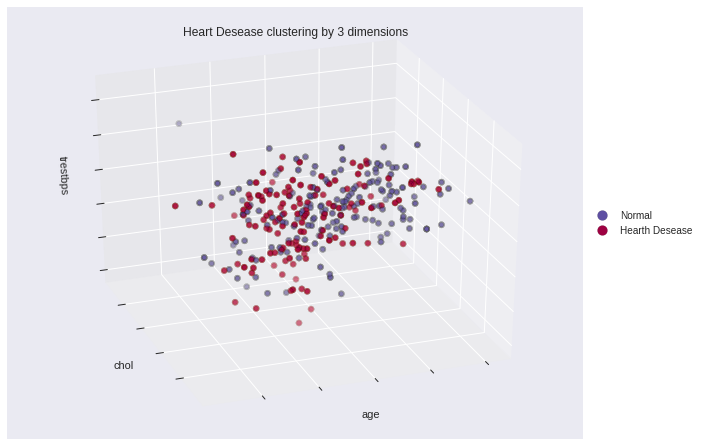
\includegraphics[width=\textwidth]{img/3d-selected.png}
    \caption{3D graph of the selected dimensions.}
\end{figure}

\section*{Applying PCA On Dataset}

Principle Component Analysis can be compute by computing standard matrix factorization technique called \textit{Singular Value Decomposition} (SVD) that can essentially decompose training matrix $X$ into dot product of three matrices $U \cdot \sum \cdot V^{H}$ where $V^{H}$ is the eigenvectors. 

I will be using Scikit Learn PCA class to obtain principle component analysis of the dataset. Using Scikit Learn is relatively straight forward since the library has unified API for all the algorithms. First I will start with initiating class instance then \textit{fit\_transform} method can be called on that instance while passing dataset. User can specify the \textit{n\_components} they wish to receive in the class instance as an attribute and the result of PCA will be same number of dimensions for decomposed matrix. In the fallowing example I choose '3' components and received the three dimensional decompose matrix.  

\begin{python}
    pca = PCA(n_components=3)
    df_reduced = pca.fit_transform(df[df.columns[:-1]])
    df_reduced[:5]

    array([[-12.26734484,   2.87383781,  14.96987876],
       [  2.69013712, -39.87137362,   0.8778823 ],
       [-42.95021407, -23.63681988,   1.75944589],
       [-10.94475636, -28.43803577,  -7.04418048],
       [106.97905333, -15.87446784, -14.8615748 ]])
\end{python}

Yet choosing arbitrary number for components not a good practice and do not tell us anything about nature of the decomposed matrix. It is usually more sensible to choose number of components based on the percentage of variance (e.g., 95\%) of the data. Scikit Learn has useful \textit{explained\_variance\_ratio\_} attribute available which is generated from fitting the data. This attribute give us the percentage of explained variance in each of the components of decomposition. For above example we can retrieve the expected variance.

\begin{python}
    pca.explained_variance_ratio_

    >>> array([0.7475642 , 0.15037022, 0.08459685])
\end{python}

This result tell us that the first eigenvalues of the decompose matrix explains $\approx 75\%$, second eigenvalues $\approx 15\%$ and third eigenvalues $\approx 8\%$ of the variance.

In order to choose number of components that will give us the total explained variance of 95\% we can fit a PCA instance without explicitly specifying the number of components. This instance will return us maximum number of eigenvalues available and their explained variance where we can calculate desired level of explained variance and associated number of components.

\begin{python}
    pca_search = PCA()
    pca_search.fit_transform(df[df.columns[:-1]])
    cum_sum = np.cumsum(pca_search.explained_variance_ratio_)
    confidence_degree = np.argmax(cum_sum >= 0.95) + 1
    confidence_degree

    >>> 3
\end{python}

We can observe from the example above in fact three components are enough to reach over 95\% variance in this dataset. Another way to obtain PCA values with same level of variance is to pass the ratio to PCA instance as a number of components. For example \textit{PCA(n\_components=0.95)} will also give us same result. In some cases it might be useful to visualize the number of components as a variable of explained variance and choose the desired number of components.

\begin{python}
    plt.plot(list(range(1, len(cum_sum) + 1)), cum_sum)
    plt.xlabel("Number of components")
    plt.ylabel("Explained variance")
\end{python}

\begin{figure}[H]
    \centering
    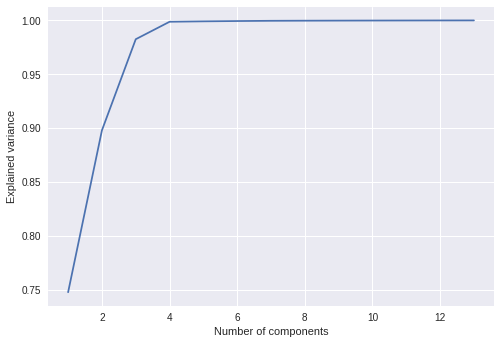
\includegraphics[width=\textwidth]{img/variance-components.png}
    \caption{Ratio of explained variance in respect to number of components.}
\end{figure}

Given that we choose the number of components, we can plot the PCA values and observe how they represent the dataset.

\begin{python}
    labelTups = [("Normal", 0), ("Hearth Desease", 1)]
    fig = plt.figure(1, figsize=(8, 6))
    ax = Axes3D(fig, elev=-150, azim=110)
    ax.scatter(df_reduced[:, 0], df_reduced[:, 1], df_reduced[:, 2], c=y,
            cmap=plt.cm.Set1, edgecolor='k', s=40)
    ax.set_title("PCA with 3 components")
    ax.set_xlabel("1st eigenvector")
    ax.w_xaxis.set_ticklabels([])
    ax.set_ylabel("2nd eigenvector")
    ax.w_yaxis.set_ticklabels([])
    ax.set_zlabel("3rd eigenvector")
    ax.w_zaxis.set_ticklabels([])

    sc = ax.scatter(df_reduced[:, 0], df_reduced[:, 1], df_reduced[:, 2], c=y, cmap="Spectral", edgecolor='k')

    colors = [sc.cmap(sc.norm(i)) for i in [1, 0]]
    custom_lines = [plt.Line2D([],[], ls="", marker='.', 
                    mec='k', mfc=c, mew=.1, ms=20) for c in colors]
    ax.legend(custom_lines, [lt[0] for lt in labelTups], 
            loc='center left', bbox_to_anchor=(1.0, .5))
\end{python}

\begin{figure}[H]
    \centering
    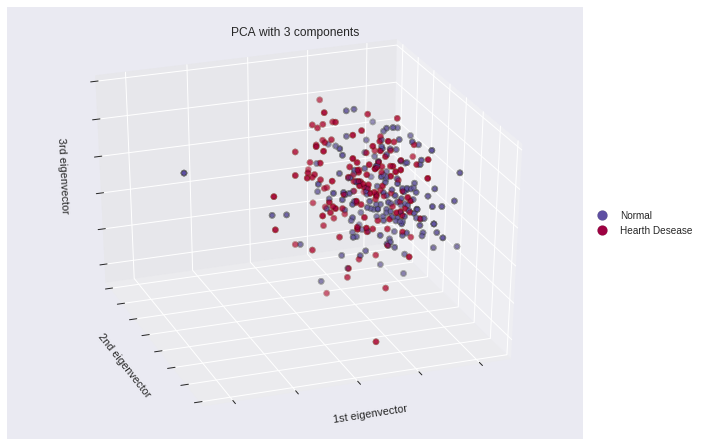
\includegraphics[width=\textwidth]{img/pca.png}
    \caption{Heart Disease dataset with reduced dimensions.}
\end{figure}

\printbibliography
\end{document}